%META {"question":"Tam giác ABC có góc A tù. Hình vẽ cho thấy đường cao hạ từ đỉnh B. Đường cao ứng với cạnh AC là đoạn nào?","options":["Đoạn BH — chân cao nằm trên phần kéo dài của cạnh AC","Không tồn tại — vì tam giác có góc tù","Đoạn AH","Đoạn BA"],"answer":0,"note":"Tam giác tù tại A → đường cao từ B rơi ra ngoài cạnh AC, nằm trên phần kéo dài của AC (phần nét đứt). BH vẫn là đường cao hợp lệ vì BH ⊥ đường thẳng AC."}
\documentclass[border=5pt]{standalone}
\usepackage{tkz-euclide}
% Màu dùng chung cho toàn bộ hình vẽ (ảnh stack với nền tối của web)
\definecolor{tminc}{RGB}{226,232,240}   % chữ + nét chính
\definecolor{tmblue}{RGB}{0,210,255}    % nhấn neon xanh
\definecolor{tmpink}{RGB}{255,0,200}    % nhấn neon hồng
\definecolor{tmgreen}{RGB}{0,255,136}   % nhấn neon xanh lá
\color{tminc}

\begin{document}
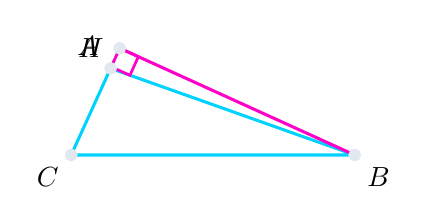
\begin{tikzpicture}[line width=1.1pt]
  \coordinate (C) at (0,0);
  \coordinate (B) at (3.6,0);
  \coordinate (A) at (0.5,1.1);
  \tkzDefPointBy[projection=onto C--A](B) \tkzGetPoint{H}
  \tkzDrawPolygon[tmblue,line width=1.1pt](A,B,C)
  \draw[tmblue,dashed] (A) -- (H);
  \draw[tmpink] (B) -- (H);
  \tkzMarkRightAngles[size=0.26,color=tmpink,line width=1pt](B,H,C)
  \tkzDrawPoints[size=3.5,color=tminc,fill=tminc](A,B,C,H)
  \tkzLabelPoint[below left=1pt](C){$C$}
  \tkzLabelPoint[below right=1pt](B){$B$}
  \tkzLabelPoint[above left=1pt](A){$A$}
  \tkzLabelPoint[left=2pt](H){$H$}
\end{tikzpicture}
\end{document}
